% The set ]0,1], its interior, and its closure, on the line.
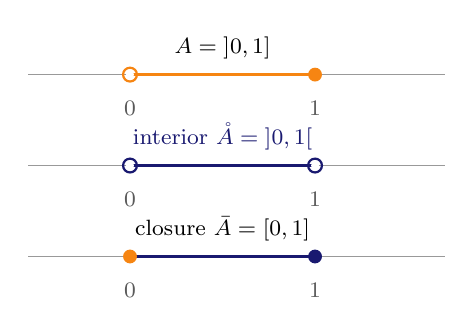
\begin{tikzpicture}[x=2.35cm,y=1.05cm,every node/.style={font=\footnotesize}]
  % A = ]0,1]
  \draw[black!40] (-0.55,2.15)--(1.7,2.15);
  \draw[BurntOrange,line width=1.2pt] (0,2.15)--(1,2.15);
  \draw[BurntOrange,line width=0.8pt] (0,2.15) circle (2.5pt);
  \fill[white] (0,2.15) circle (1.45pt);
  \fill[BurntOrange] (1,2.15) circle (2.5pt);
  \node[below,black!65] at (0,1.95) {$0$};
  \node[below,black!65] at (1,1.95) {$1$};
  \node[above] at (0.5,2.22) {$A=\mathopen]0,1]$};
  % interior
  \draw[black!40] (-0.55,1.05)--(1.7,1.05);
  \draw[MidnightBlue,line width=1.2pt] (0,1.05)--(1,1.05);
  \draw[MidnightBlue,line width=0.8pt] (0,1.05) circle (2.5pt);
  \fill[white] (0,1.05) circle (1.45pt);
  \draw[MidnightBlue,line width=0.8pt] (1,1.05) circle (2.5pt);
  \fill[white] (1,1.05) circle (1.45pt);
  \node[below,black!65] at (0,0.85) {$0$};
  \node[below,black!65] at (1,0.85) {$1$};
  \node[above,MidnightBlue] at (0.5,1.12) {interior $\mathring A=\mathopen]0,1[$};
  % closure: 0 is the point the set had missed
  \draw[black!40] (-0.55,-0.05)--(1.7,-0.05);
  \draw[MidnightBlue,line width=1.2pt] (0,-0.05)--(1,-0.05);
  \fill[BurntOrange] (0,-0.05) circle (2.5pt);
  \fill[MidnightBlue] (1,-0.05) circle (2.5pt);
  \node[below,black!65] at (0,-0.25) {$0$};
  \node[below,black!65] at (1,-0.25) {$1$};
  \node[above] at (0.5,0.02) {closure $\bar A=[0,1]$};
\end{tikzpicture}
